\documentclass[aspectratio= 43]{beamer}
%\documentclass[aspectratio=169]{beamer}

\usetheme[numbering=fullbar]{focus} % Use the Focus theme supplied with the template
% Add option [numbering=none] to disable the footer progress bar
% Add option [numbering=fullbar] to show the footer progress bar as always full with a slide count

% Uncomment to enable the ice-blue theme
%\definecolor{main}{RGB}{92, 138, 168}
%\definecolor{background}{RGB}{240, 247, 255}

%------------------------------------------------
\usepackage{amsmath}
\usepackage{tikz}
\usepackage{listings}
\usepackage[export]{adjustbox}
\usepackage{wrapfig}
\usepackage{multicol}
\usepackage{booktabs} % Required for better table rules
\usepackage[utf8]{inputenc} % Required for inputting international characters
\usepackage[T1]{fontenc} % Output font encoding for international characters
\usepackage{pdfpages}
\usepackage{multicol}
%   TITLE SLIDE

\title{\centering{Presentación Final Sistema Embebidos Distribuidos}}
\subtitle{\centering{\small{Pablo Slavkin, Gonzalo Lavigna}}}
%\titlegraphic{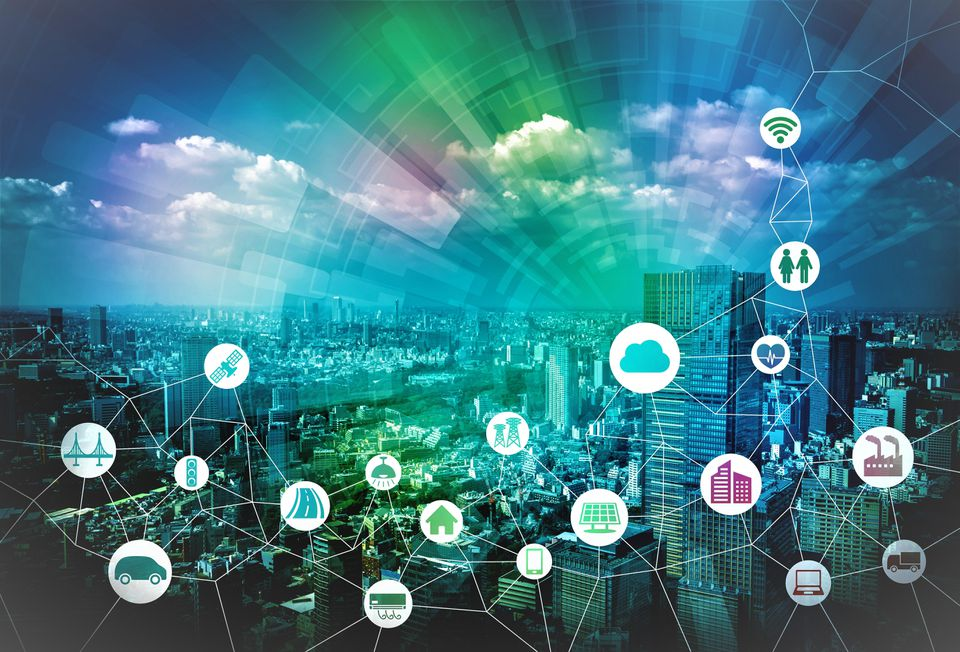
\includegraphics[scale=0.2]{Images/Connectivity.jpg}}
%\author{MESE 2019 - FIUBA}

\institute{\small{Profesores\\ Leonardo Carducci \\ Sebastian García Marra \\ Federico Zacchigna}}
\date{\small{Fecha \\ 18/10/2019 }}
%------------------------------------------------
\begin{document}

\begin{frame}
   \maketitle % Automatically created using the information in the commands above
   \begin{picture}(1,1)
      \put(240,265) {
         \hbox {
            
\includegraphics[trim=18mm  7mm  18mm 40mm,clip, width=0.3\textwidth]{./Figures/logo_fiuba.pdf}
         }
      }
   \end{picture}
\end{frame}


\begin{frame}{Motivación}
   \begin{columns}
      \column{0.4\textwidth}
      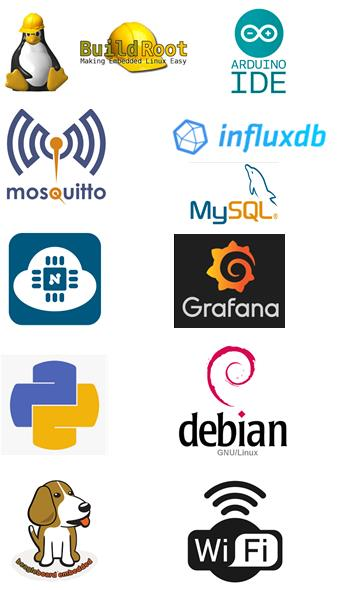
\includegraphics [width=\textwidth]{./visio/Filmina_2.jpg}
      \column{0.6\textwidth}
      \begin{itemize}
       \item{Generar un ejemplo práctico con las siguientes caracteristicas}
      \begin{itemize}
                   \item{Instanciar broker MQTT en una SBC.}
	         \item{Comunicación entre 2 redes wifi a través de la nube.}
	         \item{Utilización de bases de datos.}
	         \item{Utilización de un visor de telemetría.}
	         \item{Implementación con distintas plataformas de HW.}
      \end{itemize}
      \end{itemize}
   \end{columns}
\end{frame}

\begin{frame}{Buildroot-MySQL-Grafana-BBB wireless}
	\centering{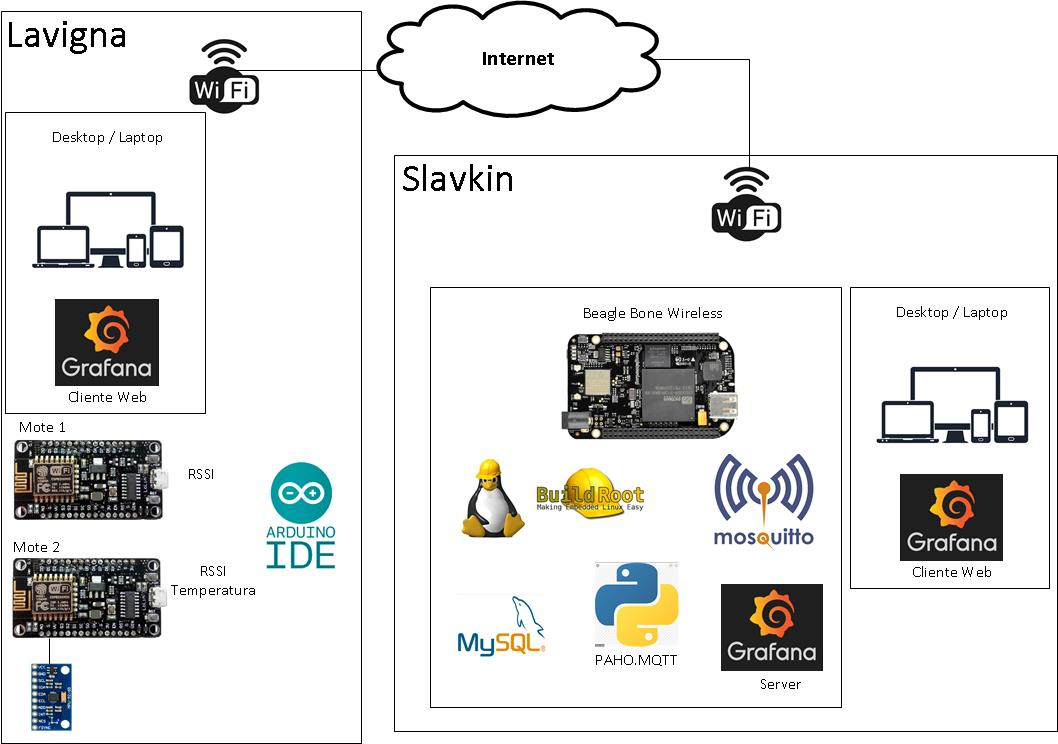
\includegraphics [scale=0.4]{./visio/Filmina_3.jpg}}
\end{frame}

\begin{frame}{Secuencia de datos 1}
   \centering 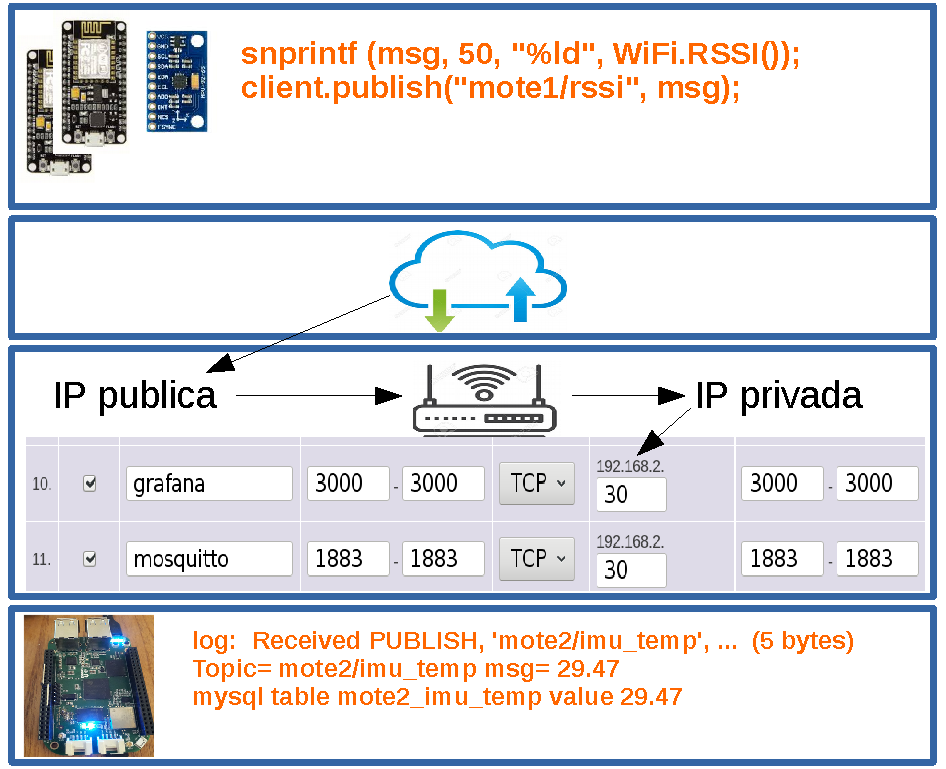
\includegraphics [scale=0.62,page=1]{./visio/secuence.pdf}
\end{frame}
\begin{frame}{Secuencia de datos 2}
   \centering \includegraphics [scale=0.62,page=2]{./visio/secuence.pdf}
\end{frame}
\begin{frame}{Secuencia de datos 3}
   \centering \includegraphics [scale=0.62,page=3]{./visio/secuence.pdf}
\end{frame}
\begin{frame}{Secuencia de datos 4}
   \centering \includegraphics [scale=0.62,page=4]{./visio/secuence.pdf}
\end{frame}
\begin{frame}{Secuencia de datos 5}
   \centering \includegraphics [scale=0.62,page=5]{./visio/secuence.pdf}
\end{frame}

\begin{frame}{Buildroot-MySQL-Grafana-BBB wireless}
 \begin{itemize}
     \item{Implementación:}
      \begin{itemize}
               \item{Mote 1 y Mote 2 se publica por MQTT el RSSI.}
               \item{Mote 2 se conecta un MPU9250 y utilizando la correspondiente libreria en Arduino IDE se publica la temperatura del die.}
               \item{A traves de Internet se conectan los motes al broker MQTT que esta en la BBB Wireless conectado dci.ddns.net.}
	    \item{Utilizando la implementación linux de ISO II se contruye con buildroot una distribución con MySQL, Mosquitto y Python.}
	    \item{Cuando se compila con buildroot se agregan al interprete de Python los package para un cliente MySQL y MQTT.}
               \item{Se realizan scripts de Python para poder guardar los datos desde el broker MQTT a las tablas de la base de datos MySQL.}
               \item{El grafana se instala utilziando el binario ARM provisto en la sección de descarga de la aplicación.}
               \item{Los dashboards del grafaba se realizan conentandonos a la BBB wireless y utilizando el cliente Web.}
      \end{itemize}
  \end{itemize}
\end{frame}


\begin{frame}{InfluxDB-Grafana-Desktop}
	\centering{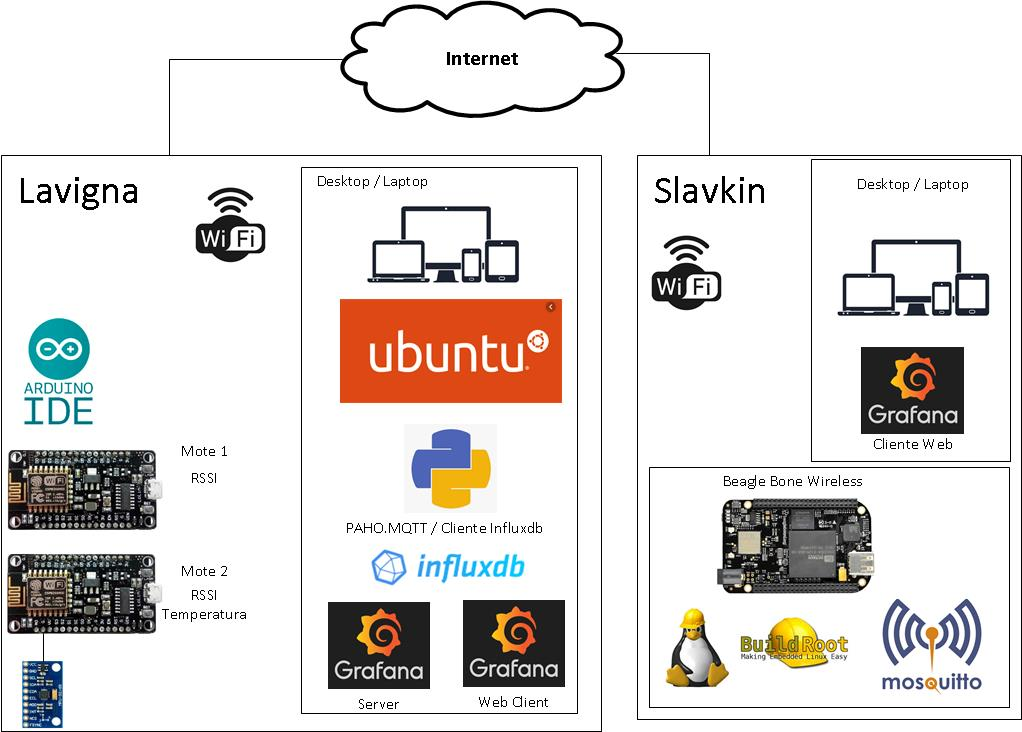
\includegraphics [scale=0.4]{./visio/Filmina_5.jpg}}
\end{frame}


\begin{frame}{InfluxDB-Grafana-Desktop}
   \begin{columns}
      \column{0.6\textwidth}
      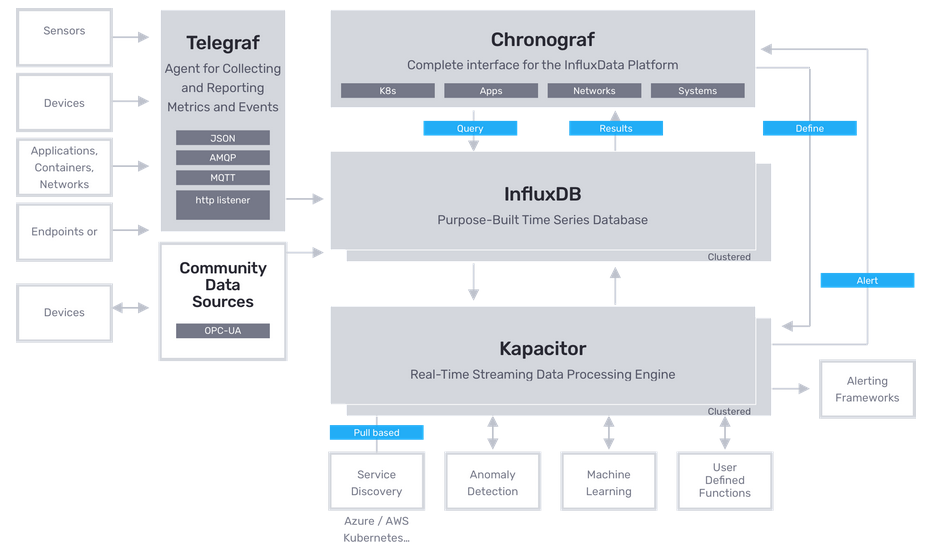
\includegraphics [scale = 0.2 ]{./Images/TICS.png}
      \column{0.5\textwidth}
      \begin{itemize}
       \item{Caracteristicas InfluxDB:}
        \begin{itemize}
               \item {Open source}
               \item {Diseñada para manejar metricas, eventos o mediciones que son time-stamped.}
               \item {Querys similares a SQL, especializadas para obtener rangos de timepos.}
               \item {API via HTTP puerto 8086 o JSON.}
               \item {Es parte del entorno TICS.}
        \end{itemize}
    \end{itemize}
   \end{columns}
  \end{frame}


\begin{frame}{InfluxDB-Grafana-BBB}
	\centering{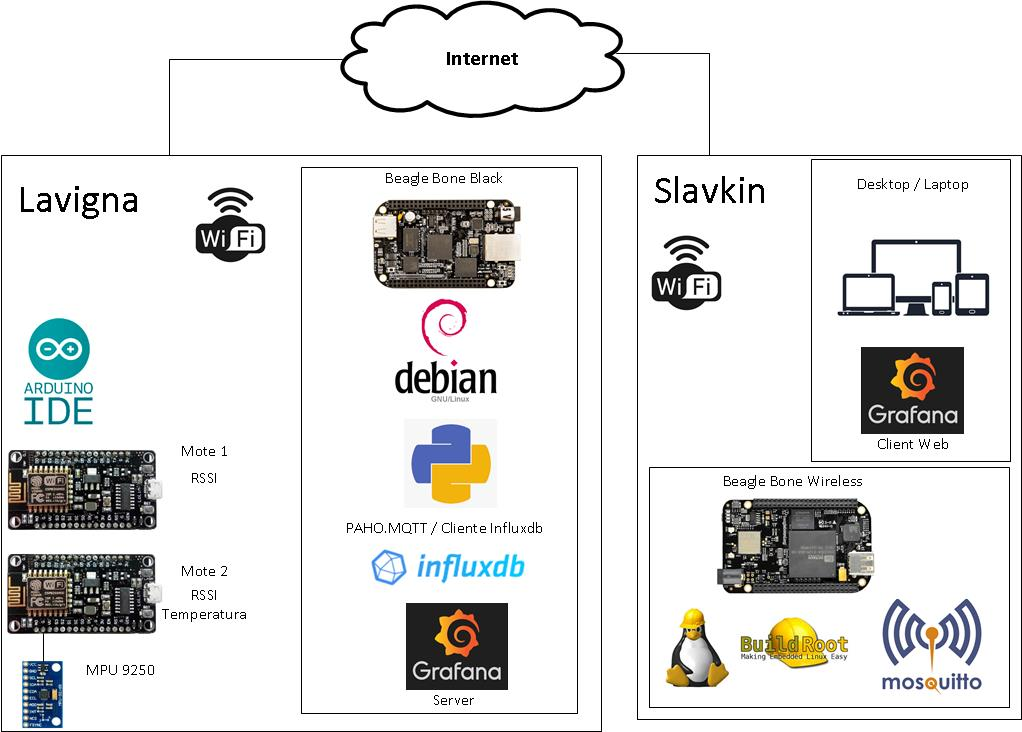
\includegraphics [scale=0.4]{./visio/Filmina_7.jpg}}
\end{frame}

\begin{frame}{Grafana}
	\centering{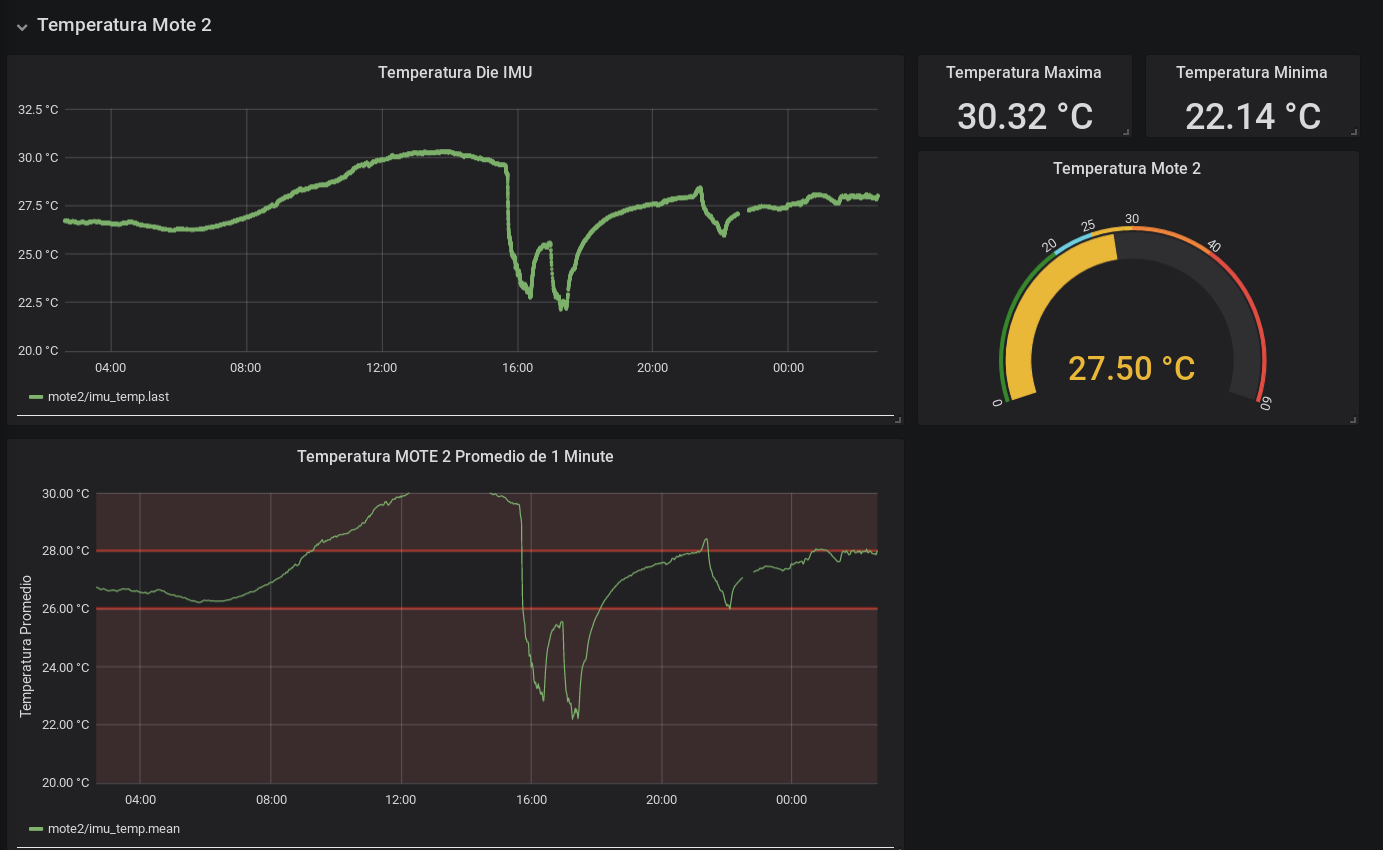
\includegraphics [scale=0.22]{./Images/Grafana_1.png}}
\end{frame}

\begin{frame}{Grafana}
	\centering{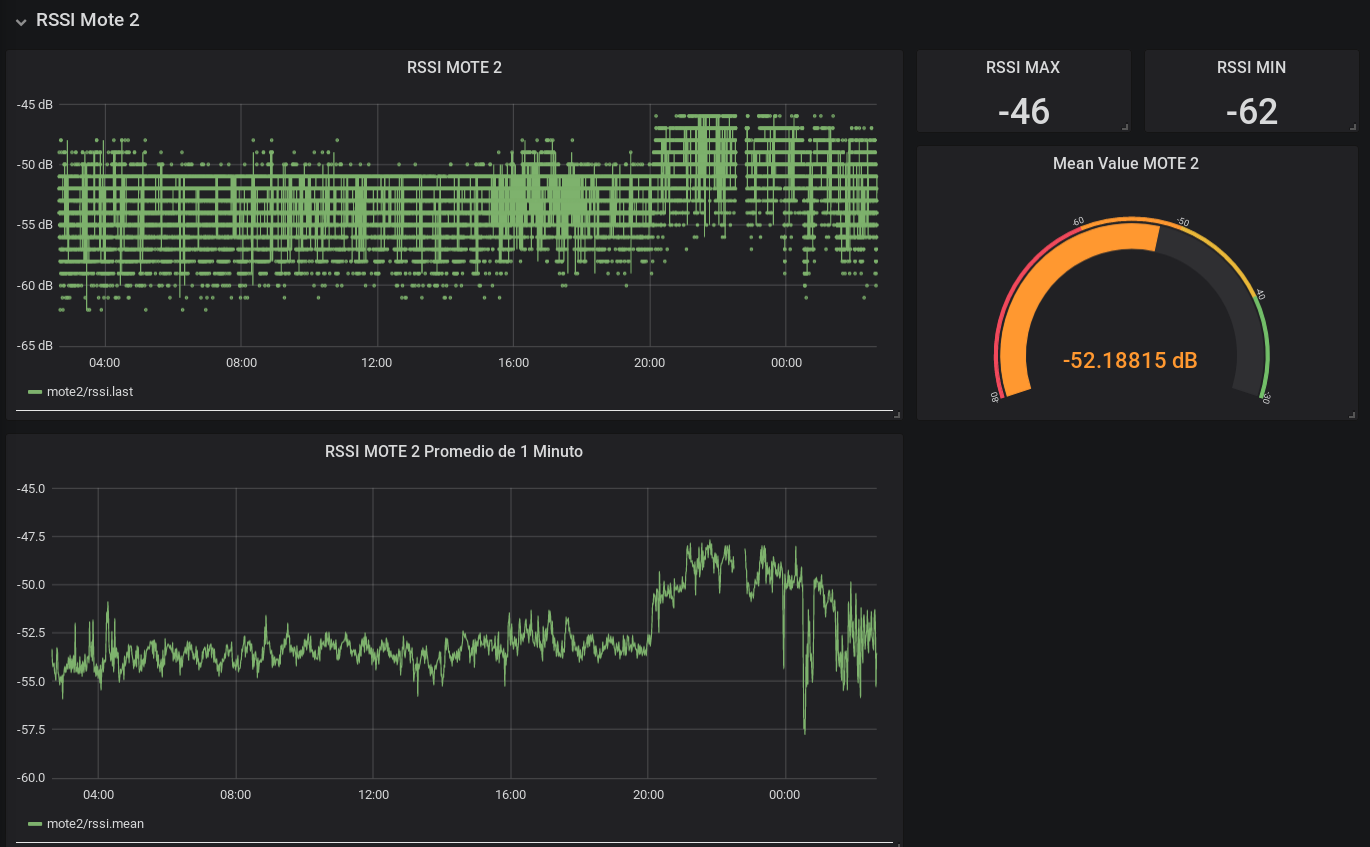
\includegraphics [scale=0.22]{./Images/Grafana_2.png}}
\end{frame}

\begin{frame}{Grafana}
	\centering{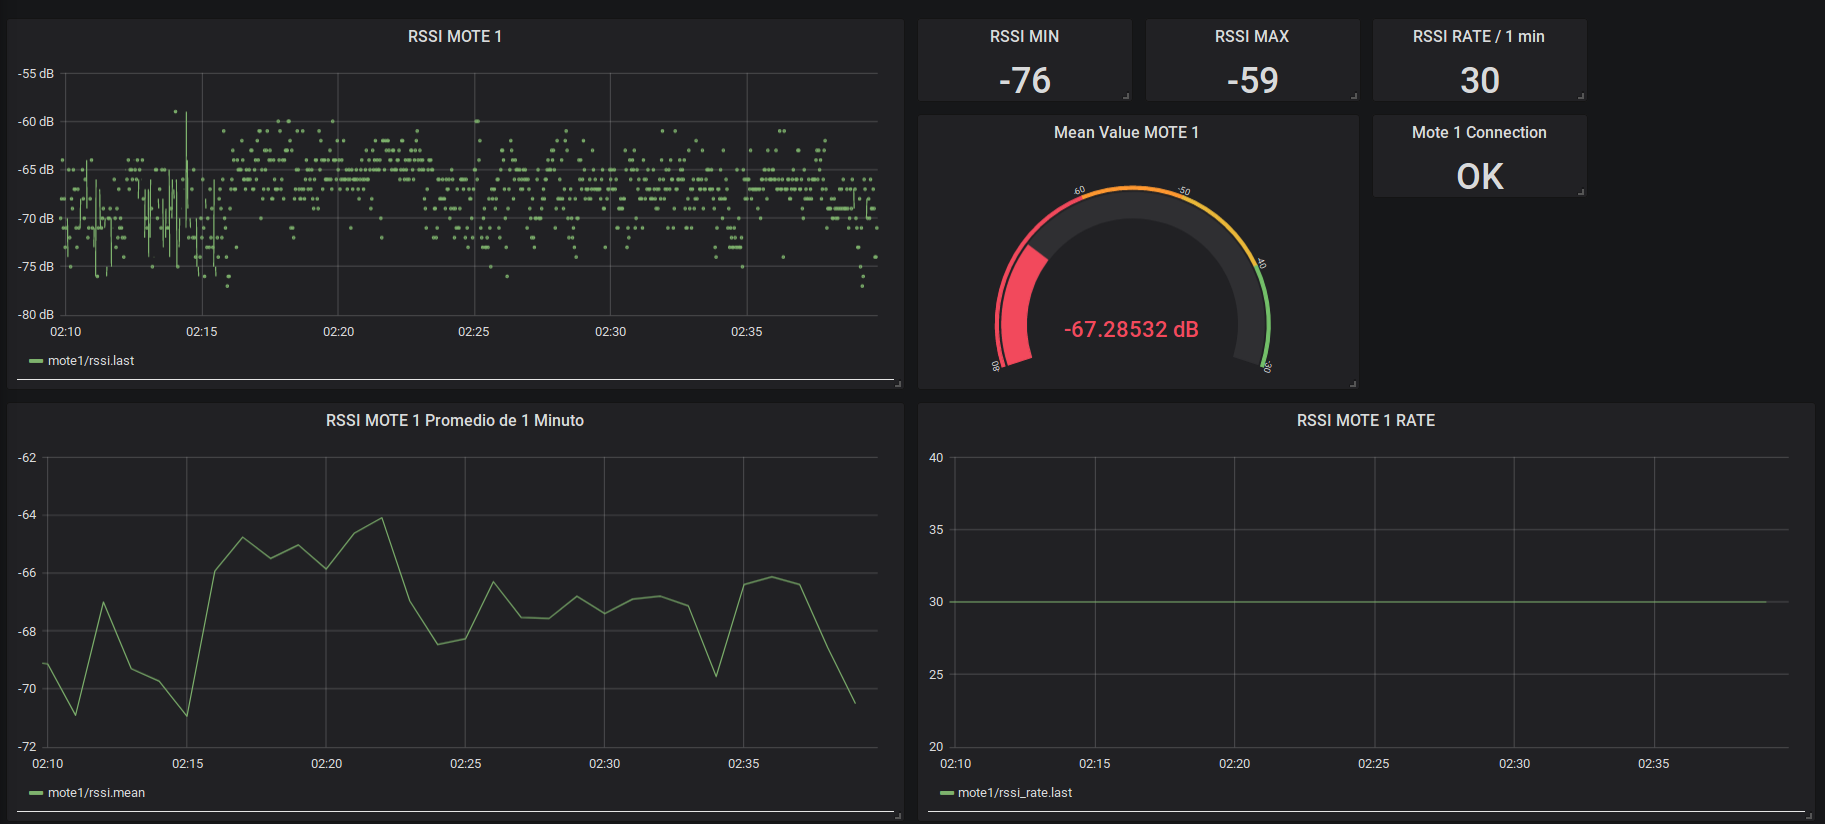
\includegraphics [scale=0.18]{./Images/Grafana_3.png}}
\end{frame}


\begin{frame}{Conclusiones - Motes}
      \begin{multicols}{2}
			ESP:
			\begin{itemize}
            \item Econimico y aseguible
            \item Bibliotecas disponibles para MQTT
            \item Bajo consumo y dimensiones reducidas
            \item Compatible con herramientas de Arduino
            \item Limitada potencia de calculo
			\end{itemize}

			\columnbreak

			Begale:
			\begin{itemize}
            \item Costo razonabe 
            \item Funcionamiento como mote/mqtt/webserver
            \item Herramientas de programacion open y estandard
            \item Herramientas de programacion open
            \item Bajo consumo de CPU
            \item Simple y agil
			\end{itemize}
      \end{multicols} 
  \end{frame}

\begin{frame}{Conclusiones - Bases de datos}
      \begin{multicols}{2}
			MySql :
			\begin{itemize}
            \item Organizacion en tablas
            \item API estandarizada
            \item Posiblidad de linkeo de tablas
            \item Estable y configurable
            \item Consumo de CPU intensivo
            \item Poco apropiada para embebidos
			\end{itemize}

			\columnbreak

			influxDB:
			\begin{itemize}
            \item Organizacion por hash tags
            \item Bajo consumo de CPU
            \item Simple y agil
            \item Configuracion limitada
            \item ?
            \item ?
			\end{itemize}
      \end{multicols} 
  \end{frame}


  \begin{frame}{Preguntas}
   \centering{
\includegraphics [scale=0.35]{./Images/preguntas.png}}
  \end{frame}

\end{document}
